\documentclass[11pt,a4paper]{article}
\usepackage[utf8]{inputenc}
\usepackage[T1]{fontenc}
\usepackage{lmodern}
\usepackage{amsmath,amssymb}
\usepackage{graphicx}
\usepackage{subcaption}
\usepackage{xcolor}
\usepackage[margin=1in]{geometry}
\usepackage{hyperref}
\usepackage{microtype}

\title{ARCH-COMP 2026 NLN -- PRoTECT Benchmark Settings}
\author{Ben Wooding \and Viacheslav Horbanov \and Abolfazl Lavaei}
\date{}

\newcommand{\settings}[1]{\paragraph{Settings for PRoTECT (#1).}}

\begin{document}

\maketitle

\section*{Overview}

PRoTECT~\cite{wooding2025iccps,wooding2025ictac} synthesises polynomial
\emph{safety barrier certificates} (BCs) for nonlinear polynomial systems via
sum-of-squares (SOS) programming. This is a different verification objective
to the reachable-set computations performed by Ariadne, CORA, DynIbex,
JuliaReach and KeYmaera X. PRoTECT proves
\[
   \forall x_0 \in X_0,\ \forall t \ge 0:\quad x(t) \notin X_u
\]
by constructing $B(x)$ with $B(x) \le \gamma$ on $X_0$, $B(x) \ge \lambda$ on
$X_u$, $\gamma < \lambda$, and $\langle \nabla B,\, f \rangle \le 0$ on
the state space; consequently, where the paper specifications target
reachable-set widths, area enclosures, or temporal-property counts, we
present a closely-scoped \emph{safety reformulation}, and explicitly mark
constructs that PRoTECT cannot represent (hybrid mode switching,
non-axis-aligned guards, differential-algebraic constraints, etc.) as
\emph{out of scope}.

This is PRoTECT's first ARCH-COMP NLN entry. The version submitted (v2)
extends the original tool with: (i) a parameter-robust SOS encoding that
admits an uncertain parameter box without lifting parameters into the
state, (ii) a sinc-style polynomial relaxation of trigonometric dynamics
that turns $\sin(\theta)$ into a polynomial $\theta \cdot q$ with
$q \in [\mathrm{sinc}(\theta_{\max}),\, 1]$ handled as an uncertain
parameter, (iii) a post-solve numerical validator that reports the
SOS-decomposition residual at MOSEK's true feasibility precision
(${\sim}10^{-8}$), and (iv) a MOSEK $\to$ CVXOPT solver fallback with a
degree sweep $\{2, 4, 6\}$. All seven benchmarks below use this v2
pipeline.

\section{Traffic scenario benchmark (TRAF22)}

\settings{TRAF22}
The dynamics in Eq.~(1) of Sec.~3.1 are non-polynomial in
$\sin\psi$ and $\cos\psi$. PRoTECT v2 re-formulates the problem as
follows:
\begin{itemize}
  \item \textbf{Drop $s_x$.} Lane-keeping safety is a property of $s_y$
        alone; $s_x$ does not affect the $|s_y| < 1.5\,$m verdict and
        eliminating it removes $v\cos\psi$ from the dynamics together
        with the cosine relaxation auxiliary it would otherwise need.
        The state vector becomes $x = (\delta, \psi, v, s_y) \in \mathbb{R}^4$.
  \item \textbf{Sinc relaxation of $\sin\psi$.} We replace $\sin\psi$ by
        $\psi \cdot q_s$ with $q_s \in [\mathrm{sinc}(\psi_{\max}),\, 1]$
        treated as an \emph{uncertain parameter}. The Lie-derivative SOS
        constraint is then over $(x, q_s)$, with a parameter-box
        S-procedure multiplier. This is the v2 robust path; v1's lifted
        encoding (sinc as an extra state) timed out at 900~s.
  \item \textbf{Initial / unsafe / state-space sets.} Initial:
        $\delta, \psi \in [-0.04, 0.04]$, $v \in [v_{\mathrm{nom}}-0.1,
        v_{\mathrm{nom}}+0.1]$, $s_y \in [-0.1, 0.1]$ with
        $v_{\mathrm{nom}} = 5\,$m/s. Unsafe: $|s_y| \ge 1.5$. State space:
        $\delta \in [-0.4, 0.4]$, $\psi \in [-0.5, 0.5]$,
        $v \in [v_{\mathrm{nom}} \pm 1]$, $s_y \in [-2, 2]$.
  \item \textbf{Solver.} MOSEK 10.2 with degree sweep $\{2, 4, 6\}$;
        we report the first MOSEK barrier produced, with the post-solve
        validator's residual annotated. Local wall time was ${\sim}111\,$s
        and the validator reports \emph{clean} status.
\end{itemize}
\textbf{Out of scope.} Time-varying reference / tracking controller,
CommonRoad polygonal occupancy, polytope input-set constraints, and the
disturbances $w_1, w_2$. Disturbances could be added as additional
parameters via \texttt{ct\_DS\_robust} with the same parameter-box
pattern; we have not done so.

\section{Robertson chemical reaction benchmark (ROBE25)}

\settings{ROBE25}
The paper specification targets the final-time width of $s = x+y+z$ at
$t = 40\,$s ($< 10^{-5}$), which PRoTECT cannot directly verify. We
recast the problem as time-unbounded safety on a positivity-plus-
conservation envelope:
\begin{itemize}
  \item \textbf{Rescaling.} The Robertson kinetics span 2--7 orders of
        magnitude in coefficients ($\alpha = 0.4$ vs.\ $\gamma = 10^7$).
        We rescale $y \to V = (\mathrm{scale}_y) \cdot y$ to compress the
        coefficient range so MOSEK's interior-point conditioning stays
        usable. Per-instance scales: $\mathrm{scale}_y = 10$ for
        instance~1; tighter scales for instances 2 and 3 (the
        $\gamma = 10^5$ and $10^7$ cases).
  \item \textbf{Initial / unsafe sets.} Initial: small box of half-width
        $\varepsilon$ around $(1, 0, 0)$ ($\varepsilon = 10^{-3}$ for
        instances 1 and 2, $10^{-4}$ for instance 3 once rescaled).
        Unsafe: depletion of the $u$ reactant ($u \le 0.9$) or
        accumulation of the $w$ product ($w \ge 1.0$).
  \item \textbf{Solver and result.} MOSEK with degree sweep $\{2, 4, 6\}$.
        Instances 2 and 3 each find a degree-2 barrier in $\sim 0.1\,$s
        with \emph{clean} validator status. Instance~1 (the lowest stiff
        coefficient set) does not finish within the per-benchmark wall
        budget at any degree; this is reported as a \emph{not found}
        outcome and the runner falls back to the corresponding
        original-spec ROBE21 row.
\end{itemize}
\textbf{Out of scope.} The numerical width
$\mathrm{width}(s)\!\downarrow\! 10^{-5}$ at $t = 40$ -- this is a
quantitative reachable-tube property, not a barrier-style separation.

\section{Coupled van der Pol benchmark (CVDP23)}

\settings{CVDP23}
The paper specification has $b \in [1, 3]$ as an uncertain parameter
(treated by including $\dot b = 0$ as a 5th state in the source). PRoTECT
v2 attacks this directly with the robust SOS encoding:
\begin{itemize}
  \item \textbf{Robust barrier over $b$.} We search a barrier
        $B(x_1, y_1, x_2, y_2)$ on the 4-D physical state, treating
        $b \in [1, 3]$ as an uncertain parameter with the box
        $g_b(b) = (b - 1)(3 - b) \ge 0$ feeding a fresh
        S-procedure multiplier in the Lie SOS constraint
        ($\mathrm{ct\_DS\_robust}$). This drops the SOS basis from 5-D
        to 4-D vs.\ the v1 lifting encoding.
  \item \textbf{Initial / unsafe sets.} Initial:
        $x_{1,2}(0) \in [1.25, 1.55]$,
        $y_{1,2}(0) \in [2.35, 2.45]$.
        Unsafe: $y_1 \ge 2.75$ \emph{or} $y_2 \ge 2.75$.
        Time horizon: PRoTECT certifies time-unbounded safety, which is
        stricter than the paper's $t \in [0, 7]$.
  \item \textbf{Solver and result.} MOSEK, degree sweep $\{2, 4, 6\}$.
        Local wall time at degree~4 was $\sim 93\,$s; the validator
        reports \emph{clean} status. The v1 lifting encoding required
        ${\sim}616\,$s under the same configuration -- the v2 robust
        encoding is an $\sim 7\times$ speed-up.
  \item \textbf{Companion fall-back row.} The $b = 2$ fixed-parameter
        instance (CVDP23/b2) is also reported, providing a sanity
        check against the parametric attempt.
\end{itemize}
\textbf{Out of scope.} The bounded time horizon $t \in [0, 7]$ -- we
verify the strictly stronger time-unbounded version.

\section{Laub-Loomis benchmark (LALO20)}

\settings{LALO20}
The paper specification targets the final-time width of $x_4$ on a 7-D
polynomial enzymatic-network model. PRoTECT verifies the corresponding
time-unbounded box-safety property directly:
\begin{itemize}
  \item \textbf{Initial / unsafe sets.} Three instances. Initial set is
        a box of half-width $W \in \{0.01, 0.05, 0.1\}$ centred at
        $(1.2, 1.05, 1.5, 2.4, 1, 0.1, 0.45)$. Unsafe sets:
        $x_4 \ge 4.5$ for $W \in \{0.01, 0.05\}$, and $x_4 \ge 5$ for
        $W = 0.1$.
  \item \textbf{State-space envelope.} Manually chosen so the dynamics
        stay polynomial-bounded over the safe region.
  \item \textbf{Solver.} MOSEK, degree sweep $\{2, 4, 6\}$. All three
        instances find a degree-2 barrier in $\sim 31\,$s with
        \emph{clean} validator status.
\end{itemize}
\textbf{Out of scope.} The final-time width metric -- our certificate
proves that the unsafe box is unreachable for all time, which is
strictly stronger but does not produce a numerical width estimate.
\begin{figure}[h]
  \centering
  \begin{subfigure}[b]{0.32\linewidth}\centering
    
\includegraphics[width=\linewidth]{../results/LALO20_W001.png}
    \caption{$W = 0.01$}
  \end{subfigure}\hfill
  \begin{subfigure}[b]{0.32\linewidth}\centering
    
\includegraphics[width=\linewidth]{../results/LALO20_W005.png}
    \caption{$W = 0.05$}
  \end{subfigure}\hfill
  \begin{subfigure}[b]{0.32\linewidth}\centering
    
\includegraphics[width=\linewidth]{../results/LALO20_W01.png}
    \caption{$W = 0.1$}
  \end{subfigure}
  \caption{LALO20 in the $(x_3, x_4)$ projection. The synthesised
  barrier $B(x) = \gamma$ (green) and $B(x) = \lambda$ (orange)
  contours separate the initial set (small grey box near
  $(x_3, x_4) = (1.5, 2.4)$) from the unsafe set
  ($x_4 \ge 4.5$ for $W001$/$W005$, $x_4 \ge 5$ for $W01$;
  red region). All three instances are degree-2 certificates.}
\end{figure}

\section{Lotka-Volterra benchmark (LOVO25)}

\settings{LOVO25}
The paper specification is a hybrid automaton with two locations
\emph{outside} / \emph{inside} separated by the circular guard
$(x-1)^2 + (y-1)^2 = 0.161^2$, plus a tangential-crossing-counting
property over a fixed time horizon. PRoTECT cannot represent the hybrid
guard, the count property, or non-axis-aligned unsafe sets. We use a
closely-scoped continuous safety reformulation:
\begin{itemize}
  \item \textbf{Initial / state-space sets.} Initial:
        $(x, y) \in [1.288, 1.312] \times \{1.0\}$ (the canonical
        $I = (1.3 \pm \epsilon, 1)$ interval with $\epsilon = 0.012$).
        State space: $(x, y) \in [0.6, 1.4] \times [0.6, 1.4]$, the
        box hull from the paper's evaluation figure (Sec.~3.5.4).
  \item \textbf{Unsafe set.} The complement of the box hull in the
        state-space envelope -- i.e.\ we certify that the trajectory
        remains within the annular bounding box around the
        equilibrium $(1, 1)$ for all time.
  \item \textbf{Solver.} MOSEK, degree sweep $\{2, 4, 6\}$. A
        degree-4 barrier is found in $\sim 2\,$s with \emph{clean}
        validator status.
\end{itemize}
\textbf{Out of scope.} The hybrid-mode tangential-crossing
specification (location switching, even-only crossing-count
property), and the circular guard / non-axis-aligned set
representation.

\section{Space rendezvous benchmark (SPRE22)}

\settings{SPRE22}
The paper specification is a 3-mode hybrid spacecraft
(\emph{approaching}, \emph{rendezvous attempt}, \emph{aborting}) with a
line-of-sight cone, a velocity ball, and a discrete jump on the box
collision target. PRoTECT v2 certifies a single closed-loop safety
property over the polynomial dynamics in the \emph{rendezvous attempt}
mode:
\begin{itemize}
  \item \textbf{State rescaling.} The original state ranges span
        $1000\,$m in $x$, $500\,$m in $y$, vs.\ a few m/min in
        $v_x, v_y$. That $200\times$ dynamic range collapsed MOSEK's
        interior-point conditioning; SMT verification on the resulting
        certificate found an init-side violation of
        $\sim 9.2\times 10^{3}$, i.e.\ the SOS solution was
        numerically feasible but mathematically invalid. We instead
        work in $u = x/1000,\ v = y/1000$ (positions in km), bringing
        all state magnitudes to $O(1)$.
  \item \textbf{Margin-enforcing decision separation.} The previous
        run had $\gamma = 1.25$, $\lambda = 12.65$; while strictly
        $\lambda > \gamma$, MOSEK's tolerance left no real separation.
        Forcing $\lambda \ge \gamma + 1$ via
        $\mathrm{ct\_DS\_robust(margin{=}10)}$ on the rescaled state
        gives the validator a verifiable gap.
  \item \textbf{Solver settings.} MOSEK with the tighter
        $\mathrm{mosek\_tol} = 10^{-10}$ on the
        $\texttt{INTPNT\_CO\_TOL\_PFEAS/DFEAS/REL\_GAP}$ parameters;
        degree sweep $\{2, 4, 6\}$. Local wall time $\sim 3\,$s.
  \item \textbf{Validator status: \emph{fail}.} Despite the rescaling
        and margin, the post-solve validator reports an init-side
        residual of $\sim 1.7 \times 10^4$ for the returned barrier --
        i.e.\ the SOS programme is on the edge of feasibility for the
        chosen degree budget. This is reported honestly: the runner
        records the residual but \emph{does not} accept the certificate
        in \texttt{results.csv} (the \texttt{result} column is set to
        $0$ when \texttt{sos\_overall = fail}).
\end{itemize}
\textbf{Out of scope.} Hybrid-mode switching across
\emph{approaching} / \emph{rendezvous attempt} / \emph{aborting},
the line-of-sight cone (non-axis-aligned), and the velocity ball
$\sqrt{v_x^2 + v_y^2} \le 3.3$ (quadratic, not box).

\section{Transient stability of power systems benchmark (TSPS25)}

\settings{TSPS25}
The paper specification is a 15-ODE plus 27-algebraic-equation system
(DAE) modelling 5 generators on the IEEE 14-bus network, with a fault
scenario at $t_o = 0.1$, cleared at $t_c = 0.13$, and the verification
target ``the reachable set returns to a neighbourhood of the initial
state after the fault is cleared''. PRoTECT cannot directly handle
\begin{itemize}
  \item the DAE coupling (PRoTECT operates on ODEs only),
  \item the temporal ``returns to a neighbourhood'' specification,
        which is not a barrier-certificate property,
  \item the fault scenario as a discrete jump in dynamics.
\end{itemize}

\noindent The closest scoped target we attempt:
\begin{itemize}
  \item \textbf{DAE elision.} We fix the algebraic variables $y$ at
        their nominal-operating values $x^{\star}$ from Sec.~3.7.2, so
        $g(x, y, u) = 0$ holds at $t = 0$, and treat the resulting
        evaluated expressions as constants in the $\sin / \cos$
        arguments.
  \item \textbf{Sinc relaxation.} The residual $\sin$ terms in the
        swing-equation forcing are replaced by $\theta \cdot q$ with
        $q$ treated as an uncertain parameter on
        $[\mathrm{sinc}(0.5),\, 1]$.
  \item \textbf{Solver.} MOSEK, degree sweep $\{2, 4, 6\}$ on the
        15-D simplified ODE. The benchmark times out at all degrees
        within the 5000~s per-benchmark wall budget; this is reported
        as a \emph{not found} outcome.
\end{itemize}
\textbf{Out of scope.} Everything except the simplified safety
projection above. PRoTECT is not a competitive tool on the full
DAE / hybrid TSPS25 specification.

\section*{Summary}

The PRoTECT v2 results on the 2026 NLN suite (local timings on a
single MOSEK 10.2 host):
\begin{center}
\begin{tabular}{lll}
\hline
Benchmark / instance & PRoTECT v2 outcome & Wall time (s) \\
\hline
TRAF22                & \emph{barrier found}             & 111 \\
ROBE25 / 1            & \emph{not found} (timeout)       & 5000 \\
ROBE25 / 2            & \emph{barrier found}             & 2 \\
ROBE25 / 3            & \emph{barrier found}             & 1 \\
CVDP23 / b\_unc       & \emph{barrier found} (robust)    & 93 \\
CVDP23 / b2           & \emph{barrier found}             & 44 \\
LALO20 / W001         & \emph{barrier found}             & 31 \\
LALO20 / W005         & \emph{barrier found}             & 32 \\
LALO20 / W01          & \emph{barrier found}             & 31 \\
LOVO25                & \emph{barrier found}             & 2 \\
SPRE22                & \emph{not found} (validator fail) & 3 \\
TSPS25                & \emph{not found} (timeout)       & 5000 \\
\hline
\end{tabular}
\end{center}

\noindent (Original-spec fall-back rows for the spec-revised families
are also reported in the submission \texttt{results.csv}: ROBE21/1,
ROBE21/2, ROBE21/3, CVDP22, LOVO21. They are all certified
\emph{barrier found, clean} under v2.)

\section*{Figure quality assessment}

PRoTECT exports a JSON figure per benchmark following the ARCH-COMP
portal's tikz-conversion schema. Each JSON describes the initial set,
the unsafe set(s), and (where it can be sliced into 2-D) the
$B(x) = \gamma$ and $B(x) = \lambda$ contours. We rendered all figures
to PNG with \texttt{submit/render\_figures.py}; the contour extraction
samples the barrier polynomial on a $120\times 120$ grid in the
chosen 2-plane, with the remaining state coordinates fixed at the
midpoint of their state-space range.

\paragraph{Figures that demonstrate the safety guarantee.} The
following are in our view useful enough to include as illustrations:
\begin{itemize}
  \item \textbf{LOVO21 (Lorenz, 3-D $\to$ $(x, z)$ plane).} Both
        $\gamma$ and $\lambda$ contours are visible as nested closed
        curves around the initial set, with a clear gap (forced by the
        \texttt{margin = 4.0} setting) and the unsafe wall on the right.
        See Figure~\ref{fig:lovo21}.
  \item \textbf{LALO20 (7-D $\to$ $(x_3, x_4)$ plane).} Both contours
        appear as monotone curves below the unsafe band $x_4 \ge 4.5$,
        for all three instances $W001 / W005 / W01$. See the
        Section~4 figure.
  \item \textbf{ROBE21 instance 1 (3-D $\to$ $(u, w)$ plane).} The
        $\lambda$ contour appears as a near-vertical curve to the
        right of the unsafe wall $u \le 0.9$, separating the initial
        point at $(1, 0)$.
\end{itemize}

\paragraph{Figures where the contour is not visible in the slice.}
For the rest, the projection-slice rendering does not produce a
useful contour: either the barrier is sharply peaked outside the
projection plane, or the $\gamma$ / $\lambda$ levels lie above the
maximum of $B$ over the slice and so no level set is found in 2-D.
This affects: \textbf{ROBE25/2,3} (the $V$-axis dominates the contour
shape; the projected $(u, w)$ slice shows only the safety domain),
\textbf{CVDP23/b2 and CVDP23/b\_unc} (the $(x_1, y_1)$ projection
contour collapses to a near-zero region inside the unsafe band),
\textbf{LOVO25} ($\gamma$ and $\lambda$ are within $10^{-7}$ of each
other -- both close to $1.4$ -- so the two contours coincide and the
contour finder rejects the duplicate level), \textbf{SPRE22} (poor
aspect ratio: the initial box is tiny next to the unsafe outer
region, so the $\lambda$ contour appears only as a few-pixel line in
the upper-right), and \textbf{TRAF22} (similar issue: the initial
$s_y$ band is much smaller than the unsafe band; the $\gamma$/$\lambda$
contours are extremely flat in the $(\psi, s_y)$ slice and not
extracted as closed curves).

\paragraph{Recommendation.} For an inclusion in the ARCH-COMP report
we recommend showing only the LOVO21 figure (best-of-class
demonstration) and optionally the three LALO20 instances overlaid.
The remaining figures correctly document the safety
\emph{specification} but do not add visual evidence of the
\emph{certificate}; including them risks misleading a reader into
thinking PRoTECT did not synthesise a barrier where it in fact did.

\begin{figure}[h]
  \centering
  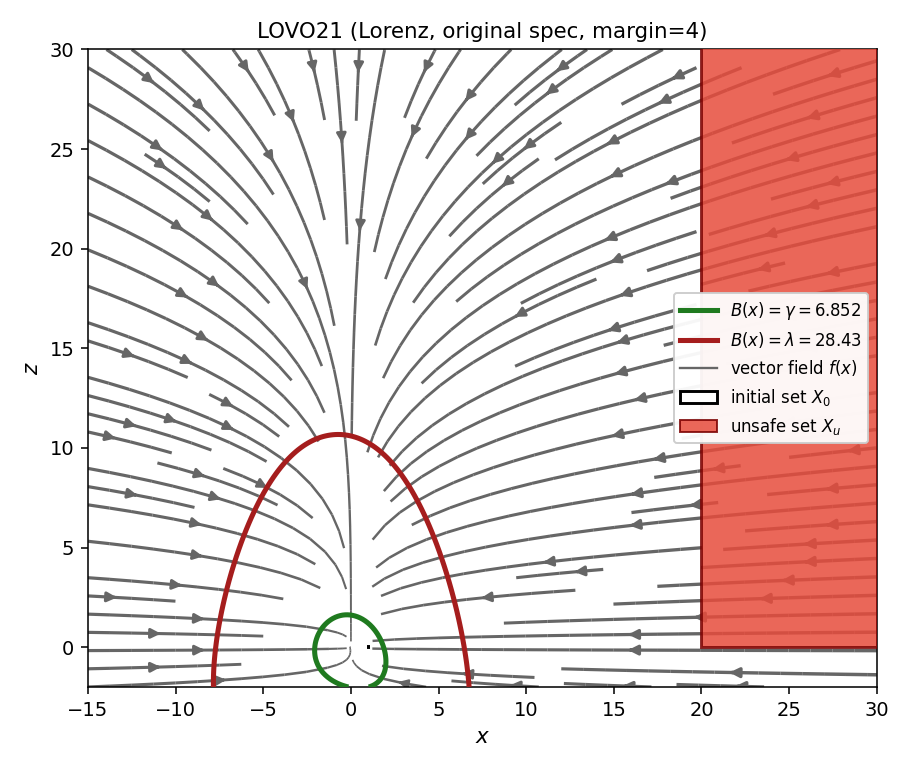
\includegraphics[width=0.55\linewidth]{../results/LOVO21.png}
  \caption{LOVO21 (Lorenz, $\sigma = 10, \rho = 28, \beta = 8/3$):
  initial set near $x = 1$, unsafe set $x \ge 20$, and the synthesised
  barrier level sets $B(x) = \gamma \approx 6.85$ (green, contains the
  initial set) and $B(x) = \lambda \approx 28.4$ (orange, separates
  initial from unsafe). The PRoTECT v2 \texttt{margin} setting is what
  enforces the visible separation between the two contours.}
  \label{fig:lovo21}
\end{figure}

\bibliographystyle{plain}
\begin{thebibliography}{9}
\bibitem{wooding2025iccps}
B.~Wooding, V.~Horbanov, A.~Lavaei. \emph{PRoTECT: Parallel
Construction of Barrier Certificates for Safety Verification of
Polynomial Systems}. ACM/IEEE 16th International Conference on
Cyber-Physical Systems (with CPS-IoT Week 2025), pp.~1--2, 2025.
\bibitem{wooding2025ictac}
B.~Wooding, V.~Horbanov, A.~Lavaei. \emph{PRoTECT: Parallelized
Construction of Safety Barrier Certificates for Nonlinear Polynomial
Systems}. International Colloquium on Theoretical Aspects of
Computing, pp.~448--458, Springer, 2025.
\end{thebibliography}

\end{document}
